
\documentclass[12pt, a4paper]{article}

\usepackage{graphicx}
\renewcommand{\refname}{5  Kaynakçalar}
\graphicspath{ {./images/} }
%opening
\usepackage{url}
\title{ Yapay Zeka Dersi Proje Tasarım Raporu}
\author{Celal ALTIN}
\date{\today}
\begin{document}
	\textbf{KÜTAHYA SAĞLIK BİLİMLERİ ÜNİVERSİTESİ}\centering\\
	\textbf{Bilgisayar Mühendisliği}\centering
	\begin{figure}[!h]
		\centering
		
\includegraphics{ksbu.png}
	\end{figure}
	\thispagestyle{empty}
	\maketitle

\maketitle\raggedright
Bu raporumda yapay zeka dersinde yapmış olduğum proje anlatılmaktadır.Raporun akışı aşağıdaki gibidir:
\begin{enumerate} 
\item Giriş
\item Literatür Araştırması
\item Metodoloji
\item Kullanılacak Veriler
\item Beklenen Sonuçlar %Sonuç
\item Kaynakça
\end{enumerate}\raggedright
\newpage
\section{Giriş}
2019 yılında başlayan COVID-19 salgını dünya çapında ciddi sağlık, ekonomik ve sosyal etkilere yol açmıştır.(Mart 2022 de yayınlanan bir habere göre \cite{haber1} dünyada ölüm sayısının 18 milyonu aştığı hesaplanıyor, bu sayı ülkemizde ise Sağlık bakanlığının verilerine göre 31.05.2022 tarihine kadar 98.965 kişinin hayatını kaybetti yönünde.)Bugün bile bu etkilerin sonuçları geçmiş değildir.\\
\begin{figure}[!htbp]
	{
	\caption{Dunya Covit Haritasi \cite{site1}}
	\centering
	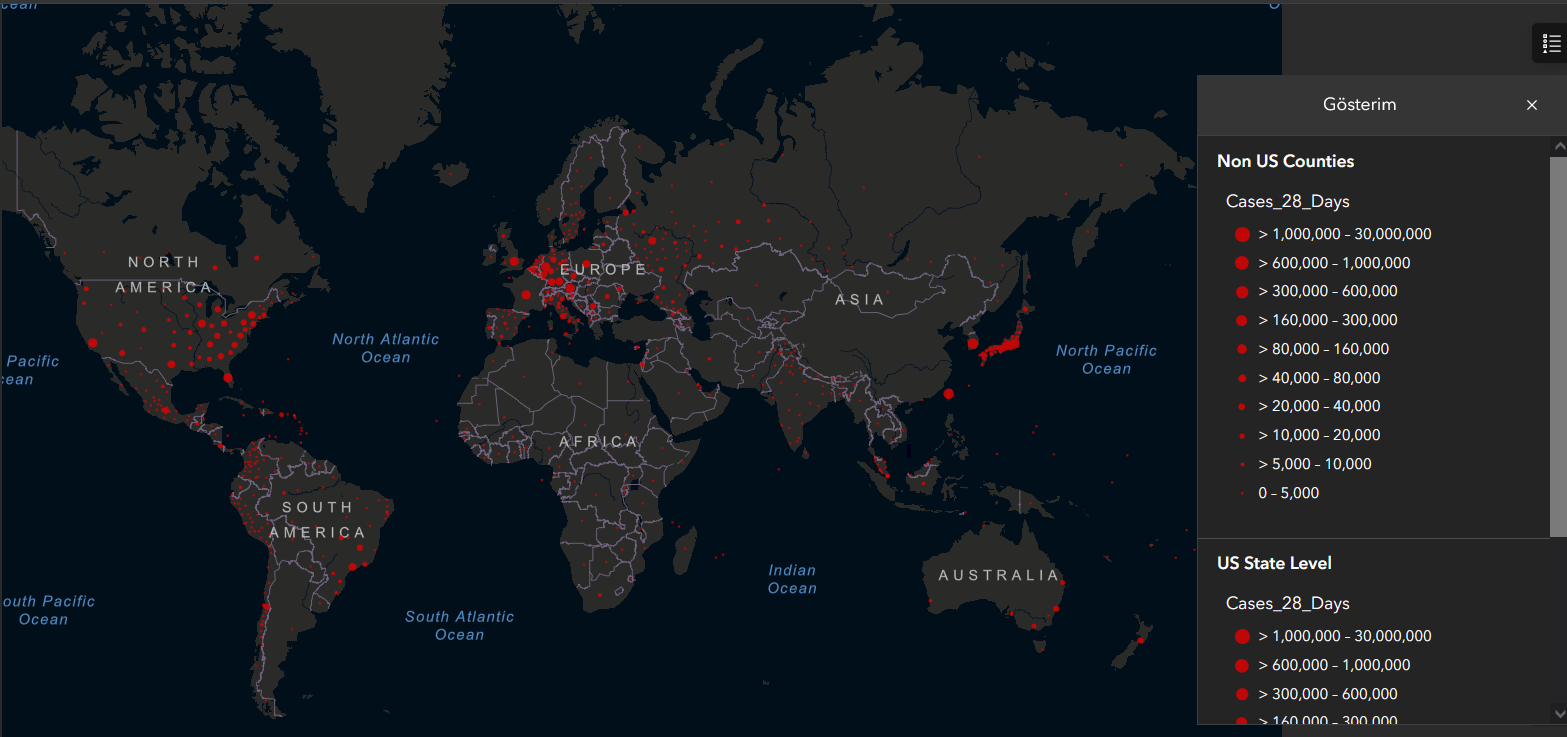
\includegraphics[angle=0, width=\textwidth]{hastalikdunya.png}
	\label{Dunya Covit Haritasi}
	}
	
	
\end{figure}
Dünya çapındaki bu problemi daha iyi anlayabilmek ve ileride olası hastalıklarda daha etkili mücadele edebilmek için bilgisayar(Makine öğrenmesi kulkanılarak yapılan bir araştırmaya göre sosyal medyanın da etkisiyle aşıya olan olumlu bakış artmıştır \cite{article} ) ve bilgisayar özelinde yapay zeka teknolojisinden faydalanmak en akılcı yöntemlerden birisidir.Bende bu projemde çeşitli kaynaklardan bulduğum Covit-19 verilerini kullanarak olası bir salgın hastalık dumunda gerçekleşebilecek seneryoyu gün yüzüne çıkartmayı amaçlıyorum.

\section{Literatür Araştırması}
Koronavirüs, 2019 yılının Aralık ayında ilk olarak Çin’in Wuhan kentinde ortaya çıkmış ve 11 Mart 2020’de Dünya Sağlık Örgütü tarafından pandemi olarak ilan edilmiştir. Vaka sayılarını kontrol altına almak için pek çok ülke karantina, sokağa çıkma yasağı ve sosyal alanların bir süreliğine kapatılması gibi çeşitli önlemler almıştır. Doğrulanmış vaka tahminlemesi pandemide olası planlamalar için büyük önem taşımaktadır. Gelecek verilerinin gerçeğe en yakın bir şekilde tahminlenmesi; pandemi döneminde lojistik, tedarik, hastane personel ve malzeme planlaması için kullanılabileceği gibi aşılama senaryolarında da girdi olarak kullanılabilir. Literatürde doğrulanmış vaka tahmininde makine öğrenmesi, bölmeli model, zaman serisi analizi gibi pek çok yöntem kullanarak tahminleme yapılan çalışmalar vardır. Bu çalışmada, Amerika Birleşik Devletleri’ndeki doğrulanmış vaka sayılarını kullanarak gelecek günlerdeki vaka tahminlerini çeşitli makine öğrenmesi modelleri yapılmıştır. Python ve R programlama dili kullanılarak yapılan tahminlemeler Prophet, Polinom Regresyon, ARIMA, Doğrusal Regresyon ve Random Forest modelleri ile yapılmıştır. Test verisiyle tahmin edilen verilerin performansları ortalama mutlak yüzde hatası (MAPE), ortalama karekök sapması (RMSE) ve ortalama mutlak hata (MAE) kullanılarak değerlendirilmiştir  \cite{article_855113}.\\ 
PCA(Veri boyutunu azaltma yöntemleri sınıflandırma yapmak için
harcanan zamanı ve bazı durumlarda sınıflandırma hatasını
azaltmaya yardımcı olur. Zaman kritik
uygulamalarda öznitelik elde etme evresinde harcanan zamanı
azaltmak için, öznitelik seçme yöntemleri, tüm giriş
değerlerinin ölçülmesini gerektiren boyut indirgeme
yöntemlerine tercih edilir\cite{genc2007new}) yöntemi kullanıldığında doğruluk değeri en yüksek RF algoritmasında,
duyarlılık ve kesinlik değeri en yüksek SMV algoritmasında saptanmıştır. Bu
yöntemin kullanılması sonucunda en düşük doğruluk NB algoritmasında,
duyarlılık ve kesinlik değerleri en düşük NB ve DT algoritmalarında elde
edilmiştir\cite{article_1031070}.
\begin{figure}[!htbp] 
	\caption{Dogruluk Tablosu}
	\centering
	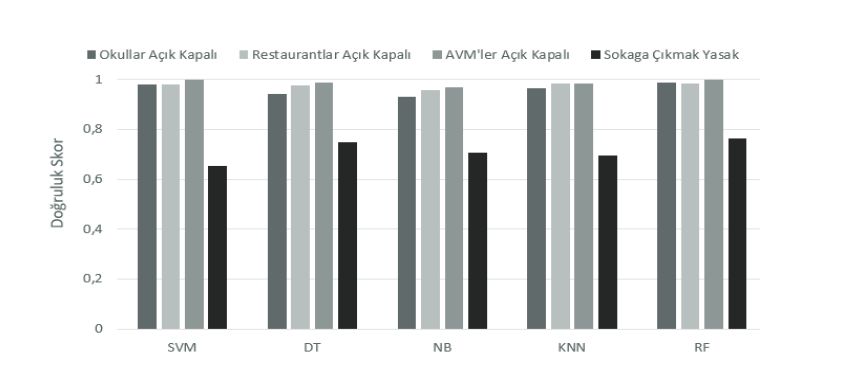
\includegraphics[angle=0, width=\textwidth]{dogruluk.png}
	\label{dogruluk}
\end{figure}
\newpage
\section{Metodoloji}
Projeni şematik planı aşağıdaki şekildedir.
\begin{figure}[!htbp]
	\caption{GANTT CHART}
	\centering
	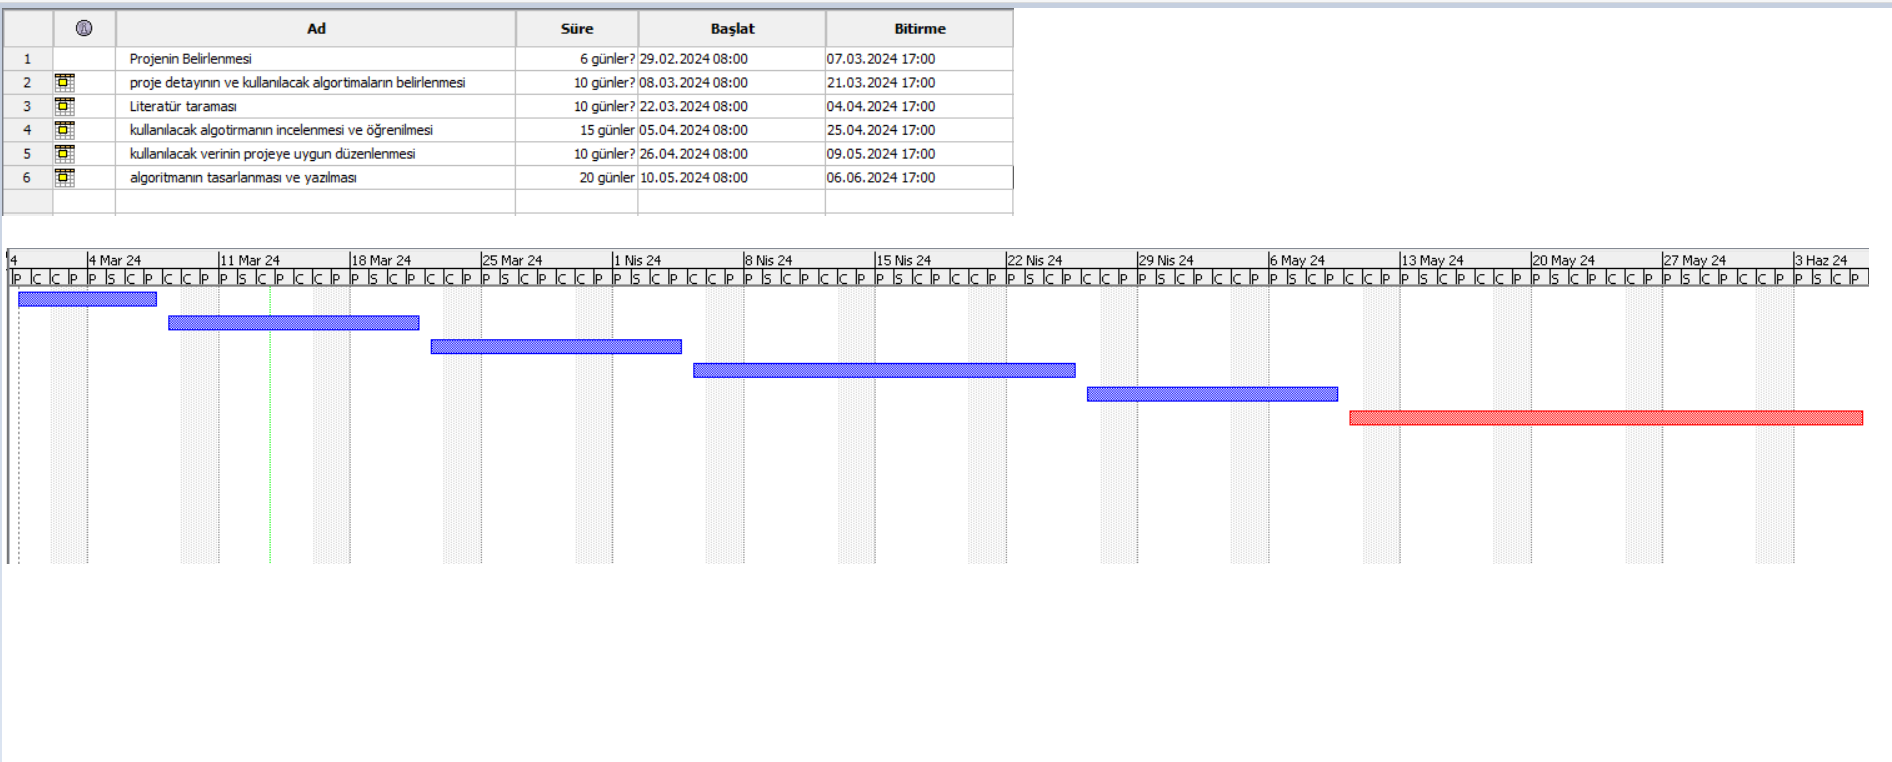
\includegraphics[ width=\textwidth]{gantt.png}
	\label{gantt}
\end{figure}

Projede kullanacağımız veriler gün veya haftalık olarak pozitif hasta sayısını, vefat edenlerin sayısını, kullandığımız verilerdeki insanların yaşadığı şehrin yada ülkenin nüfusunu, iyileşen sayısını,toplam test sayısı gibi parametreleri içermelidir.

Veri işleme
Normalizasyon işlemi- Araştırmalarda veri setlerinde verilerin
bütünlüğünün sağlanması, veri tekrarının önlenmesi ve veri bütünlüğünün
korunması ile performansının artırılması için normalizasyon yapılmaktadır.
Daha sonra Çapraz doğrulama (Çapraz doğrulama, makine öğrenimi
modellerinin başarı derecesini ortaya koymak için kullanılan yöntemdir.
Çapraz doğrulama algoritma performansı hakkında bilgi verirken, verilerin
daha verimli kullanılmasını sağlar.\cite{article_1031070})-yöntemi kullanılacaktır.
Daha sonra PCA yöntemi kullanılarak veri kümesini azalttıktan sonra RF(Random Forest) algoritmasına beslenecektir.

\section{Kullanılacak veri}


\section{Beklenen Sonuçlar}
Olası bir salgın hastalık durumunda oluşabilecek sonuçları tahmin etmede fikir vermesi ve
projemin \% 90 nın üzerinde doğrulukla sonuçlanması.
\bibliographystyle{ieeetr}
\bibliography{document.bib} 


\end{document}
